% placement.tex -- placing linear algebra on many accelerators (an idea).
% Build: latexmk (LuaLaTeX, see latexmkrc).  The numbers come from model.py
% (outputs/model.out); the program is drone.py.
\documentclass[11pt,a4paper]{article}

\usepackage{fontspec}
\usepackage{unicode-math}
\setmainfont{Libertinus Serif}
\setsansfont{Libertinus Sans}
\setmathfont{Libertinus Math}
\setmonofont{JuliaMono}[Scale=MatchLowercase]

\usepackage[margin=2.5cm]{geometry}
\usepackage{microtype}
\usepackage{booktabs,tabularx,array}
\usepackage[skip=\medskipamount]{parskip}
\usepackage{xcolor,luacolor,lua-ul}
\usepackage{listings}
\usepackage{tikz}
\usetikzlibrary{arrows.meta,fit,backgrounds,calc}
\usepackage{caption}
\usepackage[hidelinks]{hyperref}
\usepackage[nameinlink,capitalise,noabbrev]{cleveref}
\setlength{\emergencystretch}{3em}
\renewcommand{\arraystretch}{1.15}

\newcommand{\inv}{^{-1}}
\newcommand{\T}{^{\mkern-1.5mu\mathsf{T}}}
\newcommand{\invT}{^{-\mathsf{T}}}

\definecolor{kw}{HTML}{1F4E9A}
\definecolor{cm}{HTML}{6B6B6B}
\definecolor{st}{HTML}{8A3B12}
\definecolor{bg}{gray}{0.95}
\definecolor{ttbg}{gray}{0.92}
\definecolor{xfer}{HTML}{D9730D}
\let\origtexttt\texttt
\renewcommand{\texttt}[1]{\highLight[ttbg]{\origtexttt{#1}}}

\lstdefinestyle{py}{language=Python,
  basicstyle=\ttfamily\footnotesize, keywordstyle=\color{kw}\bfseries,
  commentstyle=\color{cm}\itshape, stringstyle=\color{st},
  backgroundcolor=\color{bg}, frame=none,
  xleftmargin=4pt, xrightmargin=4pt, framexleftmargin=4pt,
  framexrightmargin=4pt, aboveskip=4pt, belowskip=8pt,
  columns=fullflexible, keepspaces=true, showstringspaces=false,
  upquote=true}

% placement-styles.tex -- TikZ styles of the swimlane figures (needs the
% colours cm and xfer, and the tikz libraries arrows.meta and fit).
\tikzset{
  lane/.style={fill=black!3, draw=none},
  lanelabel/.style={font=\sffamily\small\bfseries, anchor=west},
  op/.style={draw, rounded corners=2pt, fill=blue!6, font=\sffamily\footnotesize,
    align=center, inner sep=2.5pt, minimum height=6mm},
  mat/.style={draw, fill=black!8, font=\footnotesize, inner sep=2.5pt,
    minimum height=5mm},
  io/.style={draw, rounded corners=2pt, fill=green!8, font=\sffamily\footnotesize,
    inner sep=2.5pt, minimum height=6mm},
  t/.style={font=\sffamily\scriptsize, text=cm},
  local/.style={-{Stealth[length=1.8mm]}},
  move/.style={-{Stealth[length=2.2mm]}, very thick, xfer},
  mv/.style={font=\sffamily\scriptsize, text=xfer!80!black, fill=white,
    inner sep=1pt},
  loopbox/.style={draw=cm, dashed, rounded corners=4pt},
}
% \lanes{width}: the four device lanes, CPU on top
\newcommand{\lanes}[1]{%
  \foreach \name/\y in {CPU/0, GPU/-1.5, NPU/-3, FPGA/-4.5} {
    \fill[lane] (0,\y-0.6) rectangle (#1,\y+0.6);
    \node[lanelabel] at (0.1,\y) {\name};
  }}



\title{Every Operation Where It Is Cheapest\\[0.3ex]
  \large Placing linear algebra on many accelerators, a way to cheaper AI}
\author{Michael Lehn}
\date{November 2026 \enspace·\enspace an idea for ulm.lam (Ulm Linear
  Algebra Mapping), not implemented}

\begin{document}
\maketitle

\begin{abstract}
\noindent Computers no longer have one processor. A phone, a car or a server combines
a CPU (central processing unit) with several accelerators: a GPU (graphics
processing unit), an NPU (neural processing unit), an FPGA (field-programmable
gate array), each fast at some operations and slow at others. Which
operation should run where, and when is it worth moving the data? Today
programmers decide this by hand, or a framework decides it one operation at
a time. This note proposes that a compiler decides it for the whole
program: it knows the mathematics, so it can choose the cheapest way to
compute a formula; it sees the loops, so it can move work and data out of
them; and with a cost model of the machine it can place every operation
where it is cheapest and move data only when that pays off. When the
problem size is known only at run time, the compiler generates the
competing plans and code that picks one. A made-up drone with four
processors shows the idea: for two image sizes the best plans use different
devices, and both are 10 to 50 times faster than the CPU alone.
\end{abstract}

% =====================================================================
\section{Why this makes AI cheaper}

Running an AI (artificial intelligence) model is mostly linear algebra: products of matrices and
vectors, and, in the estimation and control around the model, solving
systems of equations. What it costs, in time, in energy and in hardware,
is decided by two things: how many operations are executed, and how much
data is moved. Moving data is the expensive part: reading a number from
DRAM (dynamic random-access memory) takes on the order of a hundred times
the energy of an arithmetic operation on it~\cite{horowitz}, and moving it
between two devices costs more still.

So there are three ways to make it cheaper, and a compiler can take all
three:
\begin{itemize}
\item \emph{Fewer operations.} Use a Cholesky factorisation and triangular
  solves instead of an inverse, choose the cheapest order of a product.
  ulm.lam does this today, for BLAS (Basic Linear Algebra Subprograms)
  and LAPACK (Linear Algebra PACKage) on the CPU.
\item \emph{Each operation on the device that does it best.} A large
  product of a matrix with a vector on the NPU, a factorisation on the GPU,
  a small solve with low latency on the FPGA.
\item \emph{Data moved only when it pays off.} Moving a matrix of two
  gigabytes to the NPU is worth it for 100\,000 frames of a video, not
  for one.
\end{itemize}
Hardware that is already there is used, instead of buying a larger GPU for
everything. That is what makes it cheaper.

% =====================================================================
\section{The example: a drone}

A drone flies by camera. For every frame \(t\) it
\begin{enumerate}
\item takes an image (a vector of \(m\) pixels),
\item computes features \(f = W\,\mathit{image}\) with a linear layer \(W\)
  (\(n\times m\)), the kind of layer a neural network is made of,
\item estimates its state \(x = A\inv f\), where \(A\) (\(n\times n\)) is
  SPD (symmetric positive definite) and does not change,
\item computes the motor commands \(u = Kx\) with a controller \(K\)
  (\(k\times n\)), and steers.
\end{enumerate}
In ulm.lam's Python frontend this is the following program. It compiles
today; the generated code runs on the CPU:

\begin{lstlisting}[style=py]
camera = lam.extern("camera", [Index], Vector("m"))       # the image of frame t
steer = lam.extern("steer", [Index, Vector("k")])         # the motor commands

@lam.function
def fly(W: Matrix("n", "m"), A: Matrix("n", "n", "spd"), K: Matrix("k", "n"),
        frames: Index):
    with lam.loop(frames) as L:
        image = camera(L.index)
        f = W @ image                # features of the image: a linear layer
        x = A.inv @ f                # the estimated state of the drone
        steer(L.index, K @ x)        # the controller
\end{lstlisting}

The compiler already turns \(A\inv f\) into a Cholesky factorisation
\(A = LL\T\) and two triangular solves, and it moves the factorisation out
of the loop, because \(A\) does not change. Per frame there remain a
product with \(W\), two triangular solves with \(L\) and a product with
\(K\). The camera and the motors are attached to the CPU.

The drone has four processors. Their properties are made up, but of a
plausible magnitude (\cref{tab:devices}).

\begin{table}[h]
\centering\small
\caption{The four processors of the drone (made up). Latency in µs
(microseconds), memory bandwidth in GB/s (gigabytes per second) and
capacity in GB or MB (megabytes). A kernel takes the start-up latency plus
the larger of computing time and memory time.}
\label{tab:devices}
\begin{tabularx}{\linewidth}{@{}lXrr@{}}
\toprule
 & good at & latency & memory \\
\midrule
CPU & everything a bit; attached to camera and motors & --- & 100 GB/s \\
GPU & factorisations, large products and solves & 10 µs & 2000 GB/s, 24 GB \\
NPU & products with a large matrix that stays on chip & 40 µs & 8000 GB/s, 4 GB \\
FPGA & small products and solves, very low latency & 1 µs & 1000 GB/s, 40 MB \\
\bottomrule
\end{tabularx}
\smallskip

\raggedright\footnotesize Links from the CPU: to the GPU 25 GB/s, to the NPU 16 GB/s,
to the FPGA 8 GB/s; GPU and NPU are also linked directly (50 GB/s); other
transfers go through the CPU. The NPU cannot factorise or solve, the FPGA
cannot factorise. Matrices are in double precision.
\end{table}

% =====================================================================
\section{What the compiler decides}

For every operation the compiler chooses a device, and every value that is
used on another device than the one that computed it is transferred. The
cost of a placement is
\[
  \text{cost} = \text{once} + \mathit{frames}\cdot\text{per frame},
\]
where \emph{once} contains the factorisation and moving the matrices
\(W\), \(L\), \(K\) to where they are used, and \emph{per frame} contains
the kernels of the loop and moving the image, \(f\), \(x\) and \(u\).
A kernel on device \(d\) costs its latency plus the larger of
\(\text{operations}/\text{speed}\) and \(\text{bytes}/\text{bandwidth}\);
a transfer costs the latency of the link plus \(\text{bytes}/\text{bandwidth}\).
A matrix must fit into the memory of the device it stays on.

The compiler minimises this cost. Here there are four decisions with four
devices each, \(4^4 = 256\) placements, and it can simply try all of them
(\texttt{model.py}). For larger programs this becomes the dynamic
programming of ulm.lam's kernel selection with one more index, the device
where a value lives.

% =====================================================================
\section{Two sizes, two plans}

\paragraph{A small camera} (\(120\times120\) pixels, \(m = 14\,400\),
\(n = 900\), \(k = 16\), 100\,000 frames). The best plan uses all four
processors (\cref{fig:small}): the linear layer runs on the GPU, the
factorisation on the CPU (once), the solves and the controller on the FPGA.
\(W\) (104~MB) is moved to the GPU once; per frame only the image (115~KB
(kilobytes)) and three short vectors are moved. A frame takes 99~µs
instead of 1.05~ms (milliseconds) on the CPU alone, 10.6 times faster.

\begin{figure}[h]
\centering
% fig-small.tex -- the small-camera plan (see placement.tex)
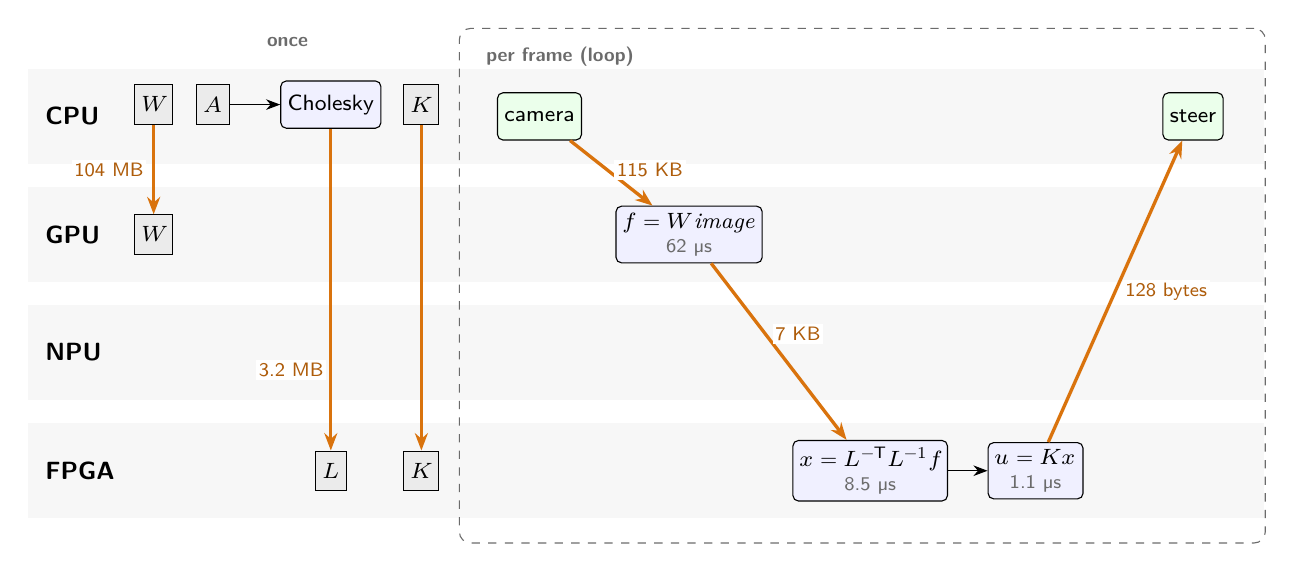
\begin{tikzpicture}[x=1cm,y=1cm]
  \lanes{15.7}
  % once
  \node[font=\sffamily\scriptsize\bfseries, text=cm] at (3.3,0.95) {once};
  \node[mat] (W) at (1.6,0.15) {\(W\)};
  \node[mat] (A) at (2.35,0.15) {\(A\)};
  \node[op] (potrf) at (3.85,0.15) {Cholesky};
  \node[mat] (K) at (5.0,0.15) {\(K\)};
  \node[mat] (Wg) at (1.6,-1.5) {\(W\)};
  \node[mat] (Lf) at (3.85,-4.5) {\(L\)};
  \node[mat] (Kf) at (5.0,-4.5) {\(K\)};
  \draw[local] (A) -- (potrf);
  \draw[move] (W) -- node[mv,left=2pt] {104 MB} (Wg);
  \draw[move] (potrf) -- node[mv,pos=.75,left=1pt] {3.2 MB} (Lf);
  \draw[move] (K) -- (Kf);
  % per frame
  \node[io] (cam) at (6.5,0) {camera};
  \node[op] (gemv) at (8.4,-1.5) {\(f = W\,\mathit{image}\)\\[-1pt]\textcolor{cm}{\scriptsize 62 µs}};
  \node[op] (trsv) at (10.7,-4.5) {\(x = L\invT L\inv f\)\\[-1pt]\textcolor{cm}{\scriptsize 8.5 µs}};
  \node[op] (ctl) at (12.8,-4.5) {\(u = Kx\)\\[-1pt]\textcolor{cm}{\scriptsize 1.1 µs}};
  \node[io] (steer) at (14.8,0) {steer};
  \draw[move] (cam) -- node[mv,pos=.45,right=2pt] {115 KB} (gemv);
  \draw[move] (gemv) -- node[mv,pos=.4,right=2pt] {7 KB} (trsv);
  \draw[local] (trsv) -- (ctl);
  \draw[move] (ctl) -- node[mv,pos=.5,right=2pt] {128 bytes} (steer);
  \node[loopbox, fit={(5.6,1.0) (15.6,-5.3)}] (loop) {};
  \node[font=\sffamily\scriptsize\bfseries, text=cm, anchor=north west] at (5.7,1.0) {per frame (loop)};
\end{tikzpicture}

\caption{Small camera: GPU, CPU and FPGA work together, 99~µs per frame.
Orange arrows move data between devices. Matrices moved once stay on
their device for all frames. \(f\) goes from the GPU to the
FPGA through the CPU.}
\label{fig:small}
\end{figure}

\paragraph{A large camera} (\(256\times256\) pixels, \(m = 65\,536\),
\(n = 4096\)). Now \(W\) has 2.1~GB. It is moved to the NPU once (134~ms)
and stays there, the GPU factorises \(A\) and keeps \(L\), and the features
go from the NPU to the GPU over their direct link (\cref{fig:large}). The
small controller runs on the CPU: for 16 commands, moving \(x\) to the FPGA
would cost more than it saves. A frame takes 0.47~ms instead of 22.8~ms on
the CPU alone, 49 times faster.

\begin{figure}[h]
\centering
% fig-large.tex -- the large-camera plan (see placement.tex)
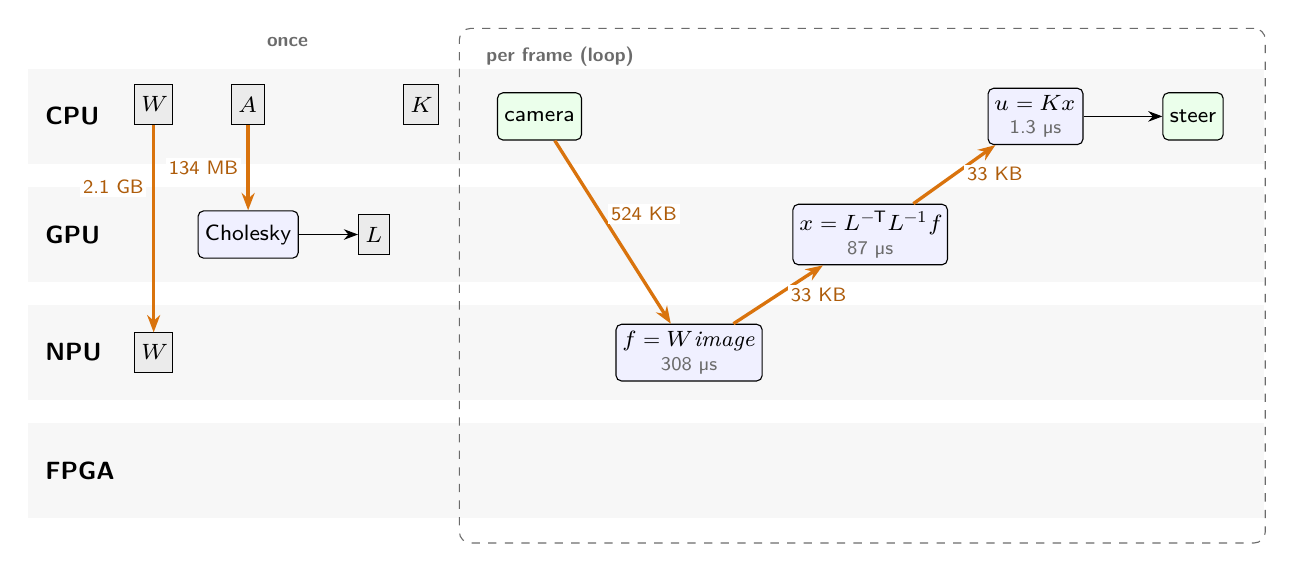
\begin{tikzpicture}[x=1cm,y=1cm]
  \lanes{15.7}
  % once
  \node[font=\sffamily\scriptsize\bfseries, text=cm] at (3.3,0.95) {once};
  \node[mat] (W) at (1.6,0.15) {\(W\)};
  \node[mat] (A) at (2.8,0.15) {\(A\)};
  \node[mat] (K) at (5.0,0.15) {\(K\)};
  \node[op] (potrf) at (2.8,-1.5) {Cholesky};
  \node[mat] (Lg) at (4.4,-1.5) {\(L\)};
  \node[mat] (Wn) at (1.6,-3) {\(W\)};
  \draw[move] (W) -- node[mv,pos=.3,left=2pt] {2.1 GB} (Wn);
  \draw[move] (A) -- node[mv,left=2pt] {134 MB} (potrf);
  \draw[local] (potrf) -- (Lg);
  % per frame
  \node[io] (cam) at (6.5,0) {camera};
  \node[op] (gemv) at (8.4,-3) {\(f = W\,\mathit{image}\)\\[-1pt]\textcolor{cm}{\scriptsize 308 µs}};
  \node[op] (trsv) at (10.7,-1.5) {\(x = L\invT L\inv f\)\\[-1pt]\textcolor{cm}{\scriptsize 87 µs}};
  \node[op] (ctl) at (12.8,0) {\(u = Kx\)\\[-1pt]\textcolor{cm}{\scriptsize 1.3 µs}};
  \node[io] (steer) at (14.8,0) {steer};
  \draw[move] (cam) -- node[mv,pos=.4,right=2pt] {524 KB} (gemv);
  \draw[move] (gemv) -- node[mv,pos=.5,right=3pt] {33 KB} (trsv);
  \draw[move] (trsv) -- node[mv,pos=.5,right=3pt] {33 KB} (ctl);
  \draw[local] (ctl) -- (steer);
  \node[loopbox, fit={(5.6,1.0) (15.6,-5.3)}] (loop) {};
  \node[font=\sffamily\scriptsize\bfseries, text=cm, anchor=north west] at (5.7,1.0) {per frame (loop)};
\end{tikzpicture}

\caption{Large camera: NPU, GPU and CPU, 0.47~ms per frame. The FPGA is
not used: \(L\) (67~MB) does not fit into its memory.}
\label{fig:large}
\end{figure}

% =====================================================================
\section{The plan is chosen at run time}

The sizes are parameters of \texttt{fly}; the compiler does not know them.
It therefore generates the plans that are best for \emph{some} sizes,
together with the comparison of their costs, which takes a few arithmetic
operations, nothing compared to a frame. ulm.lam does this today for the
order of products whose sizes are known only at run time; with devices the
costs contain latencies and bandwidths besides the numbers of operations.

As the camera grows (\(m = s^2\), \(n = s^2/16\), 100\,000 frames), the
best plan changes nine times:

\begin{center}\small
\begin{tabular}{@{}lllll@{}}
\toprule
camera from & \(f = W\,\mathit{image}\) & factorisation & solves & \(u = Kx\) \\
\midrule
\(16\times16\)   & CPU  & CPU & CPU  & CPU \\
\(56\times56\)   & FPGA & CPU & CPU  & CPU \\
\(88\times88\)   & FPGA & CPU & FPGA & CPU \\
\(96\times96\)   & GPU  & CPU & CPU  & CPU \\
\(104\times104\) & GPU  & CPU & FPGA & CPU \\
\(120\times120\) & GPU  & CPU & FPGA & FPGA \\
\(136\times136\) & NPU  & CPU & FPGA & FPGA \\
\(160\times160\) & NPU  & GPU & GPU  & CPU \\
\(304\times304\) & GPU  & GPU & GPU  & CPU \\
\(472\times472\) & CPU  & GPU & GPU  & CPU \\
\bottomrule
\end{tabular}
\end{center}

From \(304\times304\) pixels on, \(W\) no longer fits into the NPU, from
\(472\times472\) on not into the GPU either, and the product with \(W\)
returns to the CPU. The number of frames matters too. For the large camera:
\begin{itemize}
\item 1 to 4 frames: \(W\) stays on the CPU; moving 2.1~GB does not pay off.
\item 5 to 99 frames: \(W\) is moved to the GPU, which is connected faster.
\item from 100 frames on: \(W\) is moved to the NPU, which computes faster.
\end{itemize}
This is the sense of ``data is moved when it pays off'': whether a
transfer pays off depends on how often the moved data is used, and the
generated code knows that only when it is called.

Not every plan of the table needs its own code. Plans that are nearly as
good as the best one over a range of sizes can replace it, so that a few
plans cover all sizes, as for the orders of matrix products~\cite{essential}.

% =====================================================================
\section{How it fits into ulm.lam}

Most of the pieces exist:
\begin{itemize}
\item \emph{Kernel selection} chooses factorisations and solves, and the
  order of products, by dynamic programming over a cost. With devices,
  every entry of the table gets a device index, and moving a value becomes
  one more choice with a cost.
\item \emph{Moving work out of loops} is done by the LICM (loop-invariant
  code motion) pass of MLIR (Multi-Level Intermediate Representation); it
  already moves the factorisation out of the loop of \texttt{fly}.
\item \emph{Choices at run time} exist for the order of products.
\item \emph{MLIR knows devices}: memory spaces for buffers, and a dialect
  for GPUs with asynchronous copies.
\item \emph{The lowering} calls library routines (ulmBLAS, BLAS, LAPACK)
  from generated C++. The same route can call the libraries of the
  accelerators and their copy functions; the compiler itself generates no
  code for the devices.
\end{itemize}
New would be the device dimension of the selection, the transfer operation,
and above all the cost model: latencies, speeds and bandwidths of each
device and link, measured once per machine by small benchmarks.

\paragraph{Related work.} Systems that distribute a single factorisation
over CPU and GPU (MAGMA (Matrix Algebra on GPU and Multi-core
Architectures)~\cite{magma}) or schedule tasks at run time
(StarPU~\cite{starpu}) decide per operation or per task. Compilers for
neural networks place operations on devices~\cite{tarnawski}, but do not
know factorisations, solves or matrix properties. Linear algebra
compilers such as Linnea~\cite{linnea} know the mathematics, but not the
devices. Here both come together, for the whole program, including its
loops.

\paragraph{Caveat.} The drone and its processors are made up, and the
times are those of the cost model, not measurements. What the example is
meant to show: the best plan depends on the sizes and on the number of
frames, it is not obvious, and a compiler can find it.

\begin{thebibliography}{9}
\bibitem{horowitz} M.~Horowitz. Computing's energy problem (and what we can
  do about it). In \emph{IEEE (Institute of Electrical and Electronics
  Engineers) ISSCC (International Solid-State Circuits Conference)}, 2014.
\bibitem{essential} F.~López, L.~Karlsson, P.~Bientinesi. On the
  parenthesisations of matrix chains: all are useful, few are essential.
  \url{https://arxiv.org/abs/2303.17352}, 2023.
\bibitem{magma} S.~Tomov, J.~Dongarra, M.~Baboulin. Towards dense linear
  algebra for hybrid GPU accelerated manycore systems. \emph{Parallel
  Computing}, 2010.
\bibitem{starpu} C.~Augonnet, S.~Thibault, R.~Namyst, P.-A.~Wacrenier.
  StarPU: a unified platform for task scheduling on heterogeneous multicore
  architectures. \emph{Concurrency and Computation: Practice and
  Experience}, 2011.
\bibitem{tarnawski} J.~Tarnawski, A.~Phanishayee, N.~Devanur, D.~Mahajan,
  F.~Nina Paravecino. Efficient algorithms for device placement of DNN
  (deep neural network) graph operators. In \emph{NeurIPS (Conference on
  Neural Information Processing Systems)}, 2020.
\bibitem{linnea} H.~Barthels, C.~Psarras, P.~Bientinesi. Linnea: automatic
  generation of efficient linear algebra programs. \emph{ACM (Association
  for Computing Machinery) Transactions on Mathematical Software}, 2021.
\end{thebibliography}

\end{document}
